\documentclass[a4paper, 14pt]{extarticle}

% Поля
%----------------------
\usepackage{geometry}
\geometry{a4paper,left=2cm,right=1cm,
    top=2cm,bottom=2cm,bindingoffset=0cm}
%----------------------

% Russian-specific packages
%----------------------
\usepackage[T2A]{fontenc}
\usepackage[utf8]{inputenc}
\usepackage[english, main=russian]{babel}
%----------------------

\usepackage{textcomp}

% Красная строка
%----------------------
\usepackage{indentfirst}
%----------------------

% Graphics
%----------------------
\usepackage{graphicx}
\graphicspath{ {./images} }
\usepackage{wrapfig}
%----------------------

% Import minted
%----------------------
\usepackage{minted}
%----------------------

\linespread{1.3}
\sloppy
\clubpenalty=10000
\widowpenalty=10000

\begin{document}

%--------------------------------------
%			ТИТУЛЬНЫЙ ЛИСТ
%--------------------------------------
\begin{titlepage}
\thispagestyle{empty}
\newpage


%Шапка титульного листа
%--------------------------------------
\vspace*{-60pt}
\hspace{-65pt}
\begin{minipage}{0.3\textwidth}
\hspace*{-20pt}\centering

\includegraphics[width=\textwidth]{emblem}
\end{minipage}
\begin{minipage}{0.67\textwidth}\small \textbf{
\vspace*{-0.7ex}
\hspace*{-6pt}\centerline{Министерство науки и высшего образования Российской Федерации}
\vspace*{-0.7ex}
\centerline{Федеральное государственное бюджетное образовательное учреждение }
\vspace*{-0.7ex}
\centerline{высшего образования}
\vspace*{-0.7ex}
\centerline{<<Московский государственный технический университет}
\vspace*{-0.7ex}
\centerline{имени Н.Э. Баумана}
\vspace*{-0.7ex}
\centerline{(национальный исследовательский университет)>>}
\vspace*{-0.7ex}
\centerline{(МГТУ им. Н.Э. Баумана)}}
\end{minipage}
%--------------------------------------

%Полосы
%--------------------------------------
\vspace{-25pt}
\hspace{-35pt}\rule{\textwidth}{2.3pt}

\vspace*{-20.3pt}
\hspace{-35pt}\rule{\textwidth}{0.4pt}
%--------------------------------------

\vspace{1.5ex}
\hspace{-35pt} \noindent \small ФАКУЛЬТЕТ\hspace{80pt} <<Информатика и системы управления>>

\vspace*{-16pt}
\hspace{47pt}\rule{0.83\textwidth}{0.4pt}

\vspace{0.5ex}
\hspace{-35pt} \noindent \small КАФЕДРА\hspace{50pt} <<Теоретическая информатика и компьютерные технологии>>

\vspace*{-16pt}
\hspace{30pt}\rule{0.866\textwidth}{0.4pt}
  
\vspace{11em}

\begin{center}
\Large {\bf Лабораторная работа № 2a} \\ 
\large {\bf по курсу <<Языки и методы программирования>>} \\
\large <<Модель вселенной>> \\
\large Вариант 8
\end{center}\normalsize

\vspace{8em}


\begin{flushright}
  {Студент группы ИУ9-22Б Павлов И. П. \hspace*{15pt}\\ 
  \vspace{2ex}
  Преподаватель Посевин Д. П.\hspace*{15pt}}
\end{flushright}

\bigskip

\vfill
 

\begin{center}
\textsl{Москва 2023}
\end{center}
\end{titlepage}
%--------------------------------------
%		КОНЕЦ ТИТУЛЬНОГО ЛИСТА
%--------------------------------------

\newpage
\section{Цель работы}
Получение навыка работы со статическими полями и методами. Создание простой модели вселенной

\section{Условие}
Реализовать модель вселенной. Каждый элемент вселенной должен быть объектом
некоего публичного класса, который инициализируется вспомогательным публичным
классом порождающим эту вселенную. При инициализации экземпляров класса частиц
моделируемой вселенной необходимо подсчитывать количество частиц вселенной используя
статичное экземплярное поле защищенное от изменения из объектов внешних классов путем
реализации статичного метода. Сформировать исходные данные и определить необходимые
экземплярные поля для хранения состояния объектов частиц вселенной в соответствии с
условием задачи и реализовать расчет.

\section{Реализация основного класса}
{\scriptsize
\begin{minted}{java}
public class Main {

    public static void main(String[] args) {
        System.out.println("--- Тесты ---");

        Universe.addParticle(5, -2, 7);
        Universe.addParticle(9, -6, 9);
        Universe.addParticle(-16, 4, 15);

        System.out.println("Радиус-вектор: " + Universe.getVector());
        System.out.println("Количество частиц: " + Universe.getCounter());
    }
}
\end{minted}
}

\section{Реализация вселенной}
{\scriptsize
\begin{minted}{java}
public class Universe {

    private static int counter;
    private static int x, y, z;

    public Universe(){
        counter = x = y = z = 0;
    }

    private static void calcVector(Particle entity) {
        x += entity.getX();
        y += entity.getY();
        z += entity.getZ();
    }

    public static String getVector() {
        return "(" + x + ", " + y + ", " + z + ")";
    }

    public static int getCounter() {
        return counter;
    }

    public static void addParticle(int x, int y, int z) {
        Particle new_entity = new Particle(x, y, z);
        counter++;
        calcVector(new_entity);
    }

}
\end{minted}
}

\section{Реализация частицы}
{\scriptsize
\begin{minted}{java}
public class Particle {

    private final int x;
    private final int y;
    private final int z;

    public Particle(int x, int y, int z) {
        this.x = x;
        this.y = y;
        this.z = z;
    }

    public int getX() {
        return this.x;
    }

    public int getY() {
        return this.y;
    }

    public int getZ() {
        return this.z;
    }

}
\end{minted}
}

\begin{figure}[h] 
\center{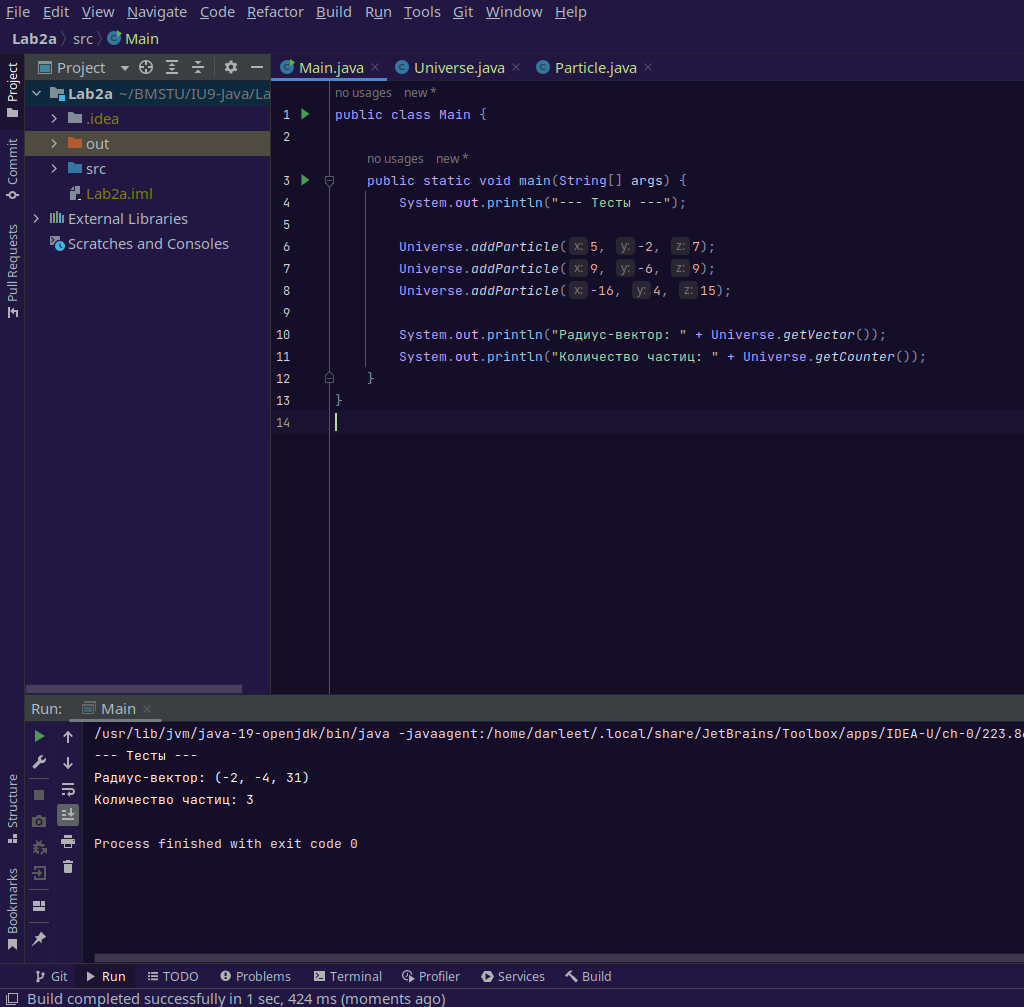
\includegraphics[scale=0.45]{class_main.png}} 
\caption{Вывод программы} 
\label{fig:image} 
\end{figure}

\end{document}
